% !TeX root = ../FoodSpy.tex
% \section{Limbaje de programare}

\section{JavaScript / TypeScript}
JavaScript este un limbaj de programare care permite implementarea unor funcționalități complexe în paginile web. Câteva dintre aceste funcționalități sunt actualizarea conținutului paginilor web în mod dinamic, animarea de grafice 2D sau 3D și afișarea hărților interactive. Alături de HTML și CSS, JavaScript este unul dintre tehnologiile web standard.
\\ \\
JavaScript este un limbaj multi-platformă, poate fi folosit pe partea de client, dar și pe partea de server, este ușor de învățat și este dinamic și flexibil. Această dinamicitate este însă și unul din dezavantajele limbajului. De exemplu, JavaScript pune la dispoziție variabile primitive de tip ”string” sau ”number”, dar pentru că nu este necesară compilarea codului, nu se verifică folosirea corectă a acestor variabile, programatorul putând folosi o variabilă ”title” pentru a reține un ”string” (Fig. \ref{fig:31}), dar care mai târziu poate va fi suprascrisă și se poate reține (în variabilă) un ”number”, fără niciun fel de avertizare din partea mediului de programare, putând conduce la bug-uri și la comportamente neprevăzute.

\begin{figure}[!htb]
	\centering
	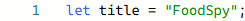
\includegraphics
	{../LaTeX/Images/ts_title-1.PNG}
	\caption{Definirea variabilei ”title”}
	\label{fig:31}
\end{figure}

Aici intervine TypeScript, un superset al limbajului JavaScript ce adaugă ”siguranța de tip” necesară pentru evitarea situațiilor neplăcute precum este cea descrisă mai sus. TypeScript încurajează scrierea codului în stil declarativ, asemănător limbajelor C\# sau Java prin facilități ca interfețe, clase și inferența de tip a variabilelor.
\\ \\
Este necesară compilarea codului scris în limbaj TypeScript, dar acest lucru poate fi văzut ca un avantaj pentru că mediul de programare poate astfel scoate în evidență comportamentul neașteptat al codului și prin urmare poate duce la detecția mult mai rapidă a bug-urilor. Referindu-ne la situația neplăcută descrisă mai sus, dacă variabila ”title” ar fi adnotată cu tipul ”string”, atunci nu va putea fi suprascrisă de o valoare pretabilă unei variabile de tip ”number”.
\newline

\begin{figure}[!htb]
	\centering
	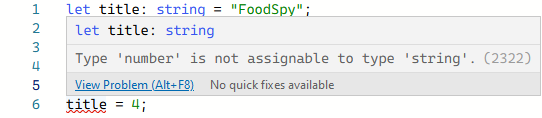
\includegraphics
	{../LaTeX/Images/ts_title-2.PNG}
	\caption{Adnotarea previne suprascrierea variabilei ”title”}
	\label{fig:32}
\end{figure}

TypeScript vine în ajutorul programatorilor care sunt deja obișnuiți cu limbaje de programare cu stil declarativ și propune astfel o alternativă față de JavaScript care nu oferă niciun suport pentru ”siguranța de tip”.
\\ \\
Deși o mai bună înțelegere a limbajului JavaScript este recomandată, TypeScript se poate învăța și folosi în mod independent, fără a cunoaște toate dedesubturile JavaScript. Mai mult, un bonus pentru programatorii cu experiență în C\# este faptul că autorul limbajului TypeScript este arhitectul limbajului C\#, deci, din punct de vedere sintactic, TypeScript și C\# împărtășesc multe similitudini.

\begin{figure}[htbp]
	\centering
	%\hspace*{-2cm}
	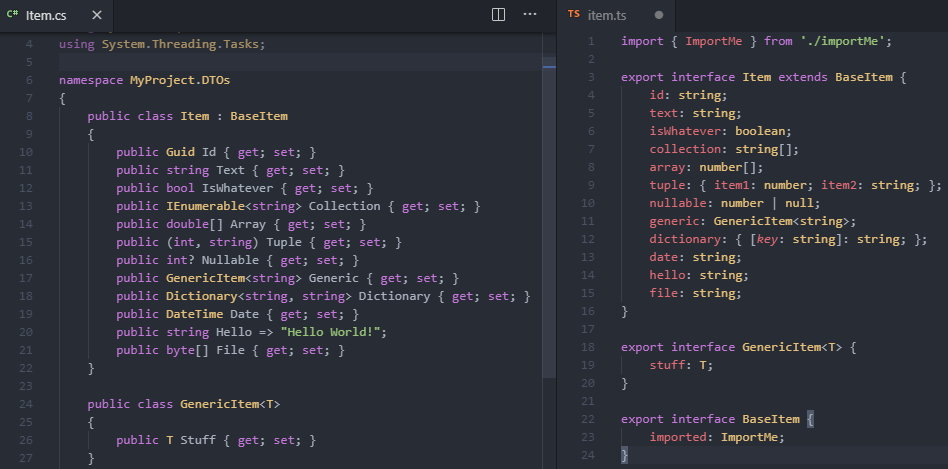
\includegraphics[width=1\textwidth]
	{../LaTeX/Images/ts_similar-3.PNG}
	\caption{Asemănări între C\# și TypeScript}
	\label{fig:33}
\end{figure}

Față de JavaScript, TypeScript întinde o plasă de siguranță care poate prinde defectele de programare introduse prin modificări majore ale codului. TypeScript nu va înlătura necesitatea depanării programelor, dar ”siguranța de tip” va ajuta fără echivoc la detectarea din timp ale defectelor. Mai mult, TypeScript beneficiază de sugestii și avertizări din partea mediului de programare încă de la compile-time, în timp ce erorile în JavaScript pot fi descoperite abia la run-time.
\\ \\
Printre alte avantaje ale TypeScript includem și posibilitatea re-factorizării într-un mod mai sigur deoarece se cunoaște codul la nivel semantic și capabilitățile TypeScript care permit construirea aplicațiilor de mărime foarte mare, în completă antiteză cu JavaScript care a fost gândit ca un limbaj folosit strict pentru modificarea dinamică a paginilor web.


\section{C\#}
C\# este un limbaj de programare orientat pe obiect, simplu, dar puternic și este gândit pentru dezvoltarea de aplicații pe platforma .NET Framework. Moștenește părțile bune ale limbajului C++ și Visual Basic, dar fără anumite inconsistențe \footnote{O astfel de inconsistență în C++ este accesul la un element dintr-un ”std::vector”. În C++ se poate folosi operatorul ”[]” pentru a ajunge la elemente care nu sunt de fapt elementele ale vectorului, ci sunt bucăți de informație conținute la adresele de memorie adiacente memoriei alocate vectorului. Deoarece nu se face niciun fel de verificare a indicelui elementului pe care încercăm să-l accesăm, operatorul ”[]” va întoarce ceea ce se află la locația de memorie vecină memoriei alocate vectorului.} și anacronisme ceea ce duc la un limbaj mai logic și mai puțin complicat.
La fel cum pentru o variabilă, simbolul ”++” înseamnă incrementarea cu 1 după ce variabila a fost evaluată, pentru C\#, simbolul ”\#” semnifică o incrementare a limbajului C++.
\\ \\
Prima versiune a apărut în 2001. Odată cu versiunea 2.0 au apărut lucrul cu generice, iteratori și metode anonime. În versiunea 3.0 au debutat metodele de extensie, expresiile lambda și cel mai important, LINQ sau Language-INtegrated Query. Versiunea 5.0 a venit cu suport nativ pentru operațiile asincron prin introducerea operatorului ”await” și modificatorului de funcție ”async”.
\\ \\
%\label{cgenerics}
Lucrul cu clase și metode generice reprezintă un concept care face posibilă proiectarea de clase și metode ale căror tipuri se cunoaște doar la momentul declarării sau instanțierii. Acest concept combină reutilizarea codului, ”siguranța de tip” și eficiența într-un mod în care nu este posibil prin proiectarea specifică.
\\ \\
”GenericList” din (Fig. \ref{fig:34}) este un exemplu de clasă generică care modelează o listă simplu înlănțuită capabilă să memoreze obiecte de tip ”Node” de orice tip, inclusiv ”int”, ”double” sau ”string”.

\begin{figure}[!htb]
	\centering
	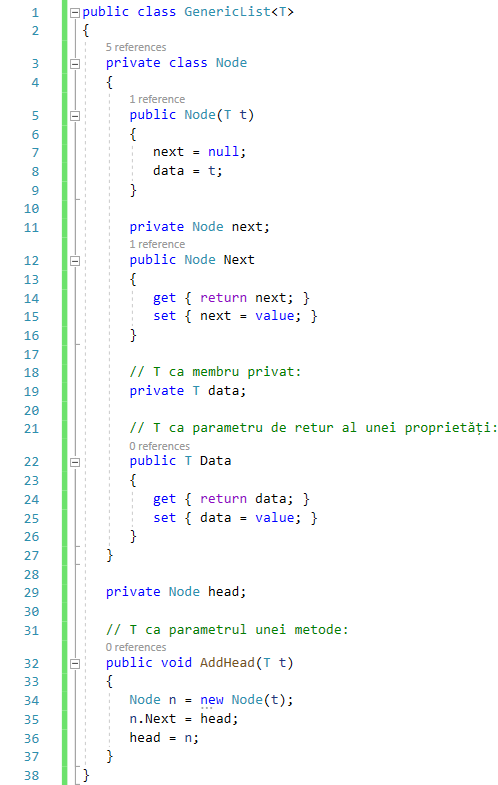
\includegraphics[width=0.8\textwidth]
	{../LaTeX/Images/csharp_generics.PNG}
	\caption{Exemplu de clasă generică}
	\label{fig:34}
\end{figure}

Parametrul de tip ”T” ia locul declarării tipului explicit și este folosit ca parametru în metoda ”AddHead(T t)”, ca parametru de retur al proprietății ”Data” și ca tip de membru privat, cum este cazul membrului ”T data”. La momentul instanțierii clasei ”GenericList<T>”, fiecare apariție a lui ”T” va fi înlocuită de tipul specificat între ”<>”.
Se pot crea interfețe, clase, metode, evenimente și delegați generici.
\\ \\
%\label{cextmeth}
Metodele de extensie sunt o funcționalitate a limbajului C\# care permit adăugarea de metode tipurilor deja existente. Metodele de extensie sunt metode statice care sunt apelate ca și cum ar fi membre ale clasei, cum este de exemplu metoda ”ToString()”, membră a clasei ”Object”.
\\ \\
O metodă de extensie are cel puțin un parametru, ”this” care reprezintă obiectul curent peste care operează metoda. Din cauza aceasta, când se apelează o metodă de extensie de către un obiect, obiectul nu trebuie trimis ca parametru.
”WordCount” din (Fig. \ref{fig:35}) este o metodă de extensie care numără caracterele dintr-un obiect de tip ”string”. Se observă că ”WordCount” este definită pentru obiecte din clasa ”System.String” deoarece parametrul ”str” este prefixat de ”this string”.

\begin{figure}[!htb]
	\centering
	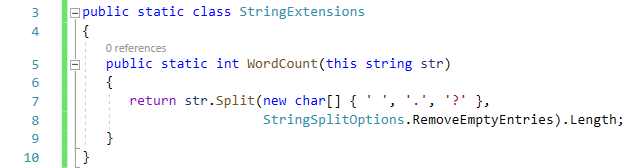
\includegraphics
	{../LaTeX/Images/csharp_extension-1.PNG}
	\caption{Exemplu de metodă de extensie}
	\label{fig:35}
\end{figure}

Apelul metodei de extensie se poate observa în (Fig. \ref{fig:36}).

\begin{figure}[!htb]
	\centering
	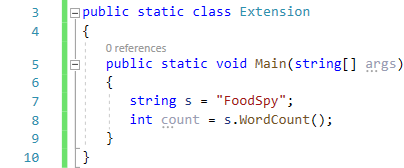
\includegraphics
	{../LaTeX/Images/csharp_extension-2.PNG}
	\caption{Apelul unei metode de extensie}
	\label{fig:36}
\end{figure}

%\label{clinq}
O definiție simplistă pentru LINQ este următoarea: modalitatea prin care se poate interoga o bază de date folosind un limbaj de interogare apropiat de SQL, dar care este compilat în interiorul unei aplicații care rulează pe platforma .NET.
Prin ”bază de date” se înțelege un spectru larg de surse de date, printre care baze de date SQL, baze de date ”in-memory” sau reprezentări XML.
\\ \\
LINQ permite scrierea unei interogări sub forma unei structuri SQL, după cum se poate observa în (Fig. \ref{fig:37}). Această structură are avantajul că variabila ”name” este ”scoped”, adică nu trebuie definită din nou pentru fiecare clauză din interogare.

\begin{figure}[!htb]
	\centering
	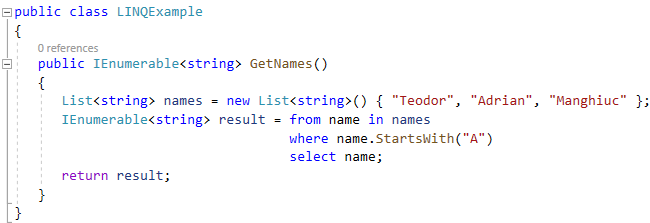
\includegraphics
	{../LaTeX/Images/csharp_linq-1.PNG}
	\caption{Exemplu de interogare LINQ}
	\label{fig:37}
\end{figure}

Un alt avantaj este claritatea originii variabilei ”name” - chiar din primul rând ("from name in names") se distinge faptul că ”name” provine din sursa de date ”names”, spre deosebire de interogarea SQL clasică, unde clauza ”from” ar fi fost declarată ultima.

LINQ nu ar fi fost un concept realizabil dacă nu s-ar fi implementat în prealabil funcționalități precum metodele de extensie, tipurile anonime \footnote{List<string> names = new List<string>() \{ "Teodor", "Adrian", "Manghiuc" \};\\Din construirea unei variabile, compilatorul are la dispoziție suficiente informații pentru a pune la dispoziție un tip de date care să modeleze variabila.}, tipurile implicite \footnote{var anonymousType = names.Select(n => new \{ Name = n, Capitalized = n.ToUpper() \});\\Din inițializarea unei variabile, compilatorul are la dispoziție suficiente informații pentru a infera tipul acesteia.\\var inference = names.Select(n => n);\\devine\\IEnumerable<string> inference = names.Select(n => n);} și expresiile lambda.


\section{HTML și CSS / SCSS}
%\label{html}
Acronimul HTML vine de la Hypertext Markup Language și reprezintă limbajul care permite structurarea conținutului unei pagini web prin construirea de secțiuni, definirea de rubrici, paragrafe și link-uri.
HTML nu este un limbaj de programare, deci nu permite construirea de conținut cu funcționalitate dinamică, dar face posibilă organizarea și formatarea paginilor web, asemenea documentelor scrise în Microsoft Word.
\\ \\
HTML este format dintr-o colecție de elemente folosite pentru a ”înfășura” bucățile de conținut astfel încât să arate sau să se comporte într-un anume fel. De exemplu, folosind elementul ”<a>” putem crea un link către o altă pagină web, cu ”<i>” putem scrie înclinat, iar cu ”<h1>” putem defini o rubrică.
În (Fig. \ref{fig:38}), este ilustrat elementul ”<p>”.

\begin{figure}[!htb]
	\centering
	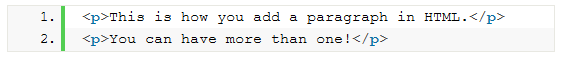
\includegraphics
	{../LaTeX/Images/html_element.PNG}
	\caption{Exemplu de element HTML}
	\label{fig:38}
\end{figure}

”p” vine de la paragraf. ”<p>” se mai numește ”opening tag” și definește punctul de intrare al elementului de tip paragraf și se poate observa că este închis între simbolurile ”<” și ”>”. ”</p>” reprezintă ”closing tag” și marchează punctul de ieșire al elementului, care, spre deosebire de punctul de intrare, mai are în componență simbolul ”/”. Textul sau conținutul paragrafului este definit între punctul de intrare și cel de ieșire. Un element HTML este format din toate cele 3 părți descrise mai sus.
\\ \\
%\label{css}
Acronimul CSS vine de la Cascading Style Sheets și reprezintă limbajul care permite determinarea aspectului unei pagini web, din punct de vedere vizual, schematic și estetic. Dacă HTML este planul unei case, CSS precizează stilul acesteia, Victorian sau Art Deco, Post-modern sau Gotic.
\\ \\
CSS schimbă aspectul paginii web interacționând cu elementele HTML. După cum am observat în (Fig. \ref{fig:38}), un paragraf este un asemenea element HTML. Dacă vrem ca textul paragrafului să fie de culoare roz și cu scris îngroșat, vom scrie codul CSS ilustrat în (Fig. \ref{fig:39}).

\begin{figure}[!htb]
	\centering
	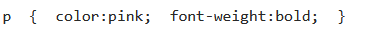
\includegraphics
	{../LaTeX/Images/css_paragraph.PNG}
	\caption{Exemplu de stilizare CSS}
	\label{fig:39}
\end{figure}

%maybe add \\ \\ here%
”p” se numește ”selector” și indică elementul HTML căruia îi vom schimba aspectul folosind reguli definite în CSS. ”color” și ”font-weight” sunt câteva dintre proprietățile de stilizare care se pot aplica selectorului de tip ”p”. Alte proprietăți ale acestuia sunt dimensiunea textului, adică ”font-size” sau ”text-transform” care poate transforma textul paragrafului în litere de tipar dacă se folosește împreună cu valoarea ”uppercase”.
\\ \\
Codul CSS poate fi adăugat unei pagini web în 3 moduri: intern, extern sau inline. În modul intern, codul CSS este scris în elementul HTML ”<style>”, ilustrat în (Fig. \ref{fig:311}).

\begin{figure}[!htb]
	\centering
	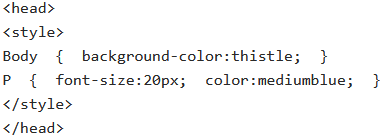
\includegraphics
	{../LaTeX/Images/css_internal.PNG}
	\caption{Modul intern de legare a codului CSS}
	\label{fig:311}
\end{figure}

Extern înseamnă scrierea codului într-un fișier separat salvat cu extensia ”.css”. Legătura dintre pagina web și regulile de stilizare din fișier se creează folosind elementul ”<link>”, după cum se poate observa în (Fig. \ref{fig:312}).

\begin{figure}[!htb]
	\centering
	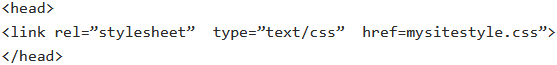
\includegraphics
	{../LaTeX/Images/css_external.PNG}
	\caption{Modul extern de legare a codului CSS}
	\label{fig:312}
\end{figure}

Codul ”inline” este codul CSS scris înăuntrul elementelor HTML, folosind proprietatea ”style”, reprezentat în (Fig. \ref{fig:313}).

\begin{figure}[!htb]
	\centering
	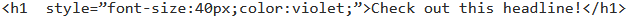
\includegraphics
	{../LaTeX/Images/css_inline.PNG}
	\caption{Modul inline de legare a codului CSS}
	\label{fig:313}
\end{figure}

Se preferă scrierea regulilor de stilizare într-un fișier separat deoarece astfel rezultă o separare între structura paginii web, elementele HTML și aspectul acesteia, regulile CSS. Codul este mai ușor de citit, mai ușor de întreținut și actualizat și permite o detectare mai ușoară a erorilor.
\\ \\
SCSS vine de la Sassy CSS și este un limbaj de preprocesare al cărui rezultat de compilare este cod CSS. În CSS este dificilă scrierea de reguli organizate și ușor de menținut deoarece lipsește suportul pentru cod imbricat (din engl. ”nested”), funcții și moștenire. Folosind SCSS se poate evita scrierea codului duplicat, prin construirea de bucăți de cod reutilizabile și se pot scrie secvențe de cod imbricate, care sunt structurate și ușor de citit (Fig. \ref{fig:314}).
\\ \\

\begin{figure}[!htb]
	\centering
	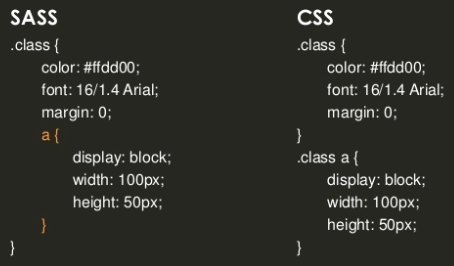
\includegraphics
	{../LaTeX/Images/scss_nesting.PNG}
	\caption{Secvență de cod ”nested”}
	\label{fig:314}
\end{figure}

Simbolul ”.” din ”.class” reprezintă o clasă de reguli de stilizare care se poate aplica unuia sau mai multor elemente HTML, spre deosebire de simbolul ”\#” care definește o regulă aplicabilă în mod unic unui singur element.
După cum se poate observa în (Fig. \ref{fig:314}), codul ”nested” evită dublarea selectorului ”.class” atunci când se face referire la elementul ”<a>”, de tip ancoră.
\\ \\
SCSS oferă suport pentru așa numitele ”directive de control”, care pot defini o regulă de stilizare dacă o anumită condiție este îndeplinită. Una dintre aceste directive este ”@if” care funcționează asemenea structurilor alternative din limbajele de programare precum C\#. Folosind ”@if”, se aplică unui element ”<div>” o margine albă de grosime de 1 pixel, dacă rezultatul condiției este egal cu 4, după cum este ilustrat în (Fig. \ref{fig:315}).

\begin{figure}[!htb]
	\centering
	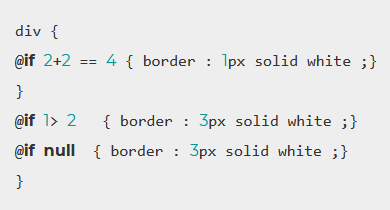
\includegraphics[width=0.4\textwidth]
	{../LaTeX/Images/scss_if-1.PNG}
	\caption{Directiva de control ”@if”}
	\label{fig:315}
\end{figure}

După evaluarea condiției din ”@if” și compilarea codului, rezultă regula de stilizare reprezentată în (Fig. \ref{fig:316}).

\begin{figure}[!htb]
	\centering
	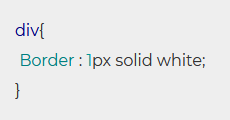
\includegraphics[width=0.2\textwidth]
	{../LaTeX/Images/scss_if-2.PNG}
	\caption{Directiva de control ”@if”}
	\label{fig:316}
\end{figure}